\documentclass[../main.tex]{subfiles}

\begin{document}
	
\chapter{Chapter 1}
\label{ch:1}

\section{Introduction}
\label{chapter1:introduction}

\section{Methods}
\label{chapter1:methods}

See progressreview 2020
Methods since then:


All data analysis and plotting was done using Python 3~\autocite{pythoncoreteamPythonDynamicOpen2020}.
The Shapiro\hyp{}Wilk normality test~\autocite{shapiroAnalysisVarianceTest1965} and Levene's homogeneity of variance~\autocite{leveneRobustTestsEquality1960} were used to test assumptions for parametric tests.
For non\hyp{}parametric analyses the Kruskal\hyp{}Wallis \textit{H} test \autocite{kruskalUseRanksOneCriterion1952} was used to test for differences between constitutive, variable and control promoters.
If necessary, Dunn's post\hyp{}hoc tests \autocite{dunnMultipleComparisonsUsing1964} were used with Bonferroni adjustment for multiple comparisons.

\subsection{Extraction of \textit{cis}-regulatory modules}\label{chapter1:methods:extraction-of-cis-regulatory-modules}

Promoters were extracted from the Arabidopsis TAIR 10 \autocite{lameschArabidopsisInformationResource2012} genome assembly and Ensembl Plants \autocite{howeEnsemblGenomes20202020} annotation (\href{ftp://ftp.ensemblgenomes.org/pub/release-47/plants/gff3/arabidopsis_thaliana/}{.gff3 release 47 date 08/03/2020}) using a custom Python script (\href{https://github.com/Switham1/PromoterArchitecture/blob/master/src/data_sorting/extract_promoter.py}{\texttt{extract\_promoter.py}}, available at \url{https://github.com/Switham1/PromoterArchitecture}).
Only promoters from genes on Arabidopsis chromosomes 1-5 were extracted.
Promoters were extracted from protein coding genes that did not overlap other protein coding genes using pybedtools \autocite{dalePybedtoolsFlexiblePython2011}.
Promoters were extracted 1000 base pairs (bp) upstream of the longest annotated transcript TSS or until the nearest annotated protein coding gene, and 5'UTRs were included downstream of the TSS up until the closest annotated coding sequence (CDS) ATG start codon.
Genes where the whole promoter overlapped a protein coding gene leaving only part of the 5'UTR non-overlapping were flagged and filtered out.
%This is because coding sequences have different conservation patterns to non-coding regions.%see intro XXX%
Promoters with an upstream gene oriented in the reverse direction less than 2000 bp away were flagged to mitigate for potentially overlapping promoters.
This was because with overlapping promoters it is difficult to determine whether CREs belong to one promoter over the other or are used by both promoters.

\subsection{Transcription factor binding site identification}
\label{chapter1:methods:transcription-factor-binding-site-identification}

The resulting promoter annotations were transformed to bed format using BEDOPS gff2bed~\autocite{nephBEDOPSHighperformanceGenomic2012},and BEDTools getfasta~\autocite{quinlanBEDToolsFlexibleSuite2010} was used to extract promoter sequences from the reference genome.
Promoters were scanned for DAP\hyp{}seq TFBS motifs~\autocite{omalleyCistromeEpicistromeFeatures2016} using FIMO~\autocite{grantFIMOScanningOccurrences2011} with a zero\hyp{}order background model created using fasta\hyp{}get\hyp{}markov~\autocite{baileyMEMESuiteTools2009}.
A \textit{p}\hyp{}value threshold of \texttildelow0.0001 and max stored sequences \texttildelow5000000 was used, and the output was filtered using a \textit{q}\hyp{}value threshold of 0.05.
Arabidopsis gene IDs for promoters and the TFs binding them were recovered for further analysis.

\subsection{Gene selection}\label{chapter1:methods:gene-selection}

To investigate the stability of expression, \textcite*{czechowskiGenomeWideIdentificationTesting2005} analysed gene expression data from \textit{Arabidopsis thaliana} Col-0 across 79 different tissues, organs, developmental stages and genotypes.
This data enables genes to be ranked according to stability of expression across tissues using coefficient of variation (CV) values.
Only genes which had at least one TFBS found in their promoters using FIMO (see \autoref{chapter1:methods:transcription-factor-binding-site-identification}) were ranked according to CV.
Recreating the methodology used by \textcite*{czechowskiGenomeWideIdentificationTesting2005}, CV was used to select the 100 most constitutively expressed genes from raw expression data generated in their study.
Alongside this, the 100 most variable genes were chosen.
100 promoters were selected from the central distribution of expression CV in the \textcite*{czechowskiGenomeWideIdentificationTesting2005} dataset.
To ensure even coverage, 10 genes were selected randomly from 10 bins covering the range of CV between the constitutive and variable gene sets.


\subsection{Sliding window creation}
\label{chapter1:methods:sliding-window-creation}
%describe how sliding windows were created%
Promoters were split into 100 bp sliding windows with a 50 bp step size using a custom Python script (\href{https://github.com/Switham1/PromoterArchitecture/blob/master/src/rolling_window/rolling_window.py}{rolling\_window.py}, available at \url{https://github.com/Switham1/PromoterArchitecture}).

\subsection{GC content}
{\label{chapter1:methods:gc-content}}

Percentage GC content of promoters and each promoter window was determined using python to test the hypothesis that constitutive genes have a higher GC content than variable genes.
%The Mann\hyp{}Whitney U test~\autocite{mannTestWhetherOne1947}


\subsection{Transcription factor binding site coverage}
{\label{chapter1:methods:transcription-factor-binding-site-coverage}}

To test the hypothesis that the CRMs of variable genes will have a lower percentage of base pairs covered by at least one TFBS than CRMs of constitutive genes, BedTools coverage tool was utilised.
The number of base pairs covered by at least one motif in a given sequence was calculated using the BEDTools coverage tool~\autocite{quinlanBEDToolsFlexibleSuite2010}.
The proportion of base pairs covered by TFBSs in constitutive promoters was compared to variable promoters using a Mann Whitney U test~\autocite{mannTestWhetherOne1947}.

\subsection{Open chromatin coverage}
{\label{chapter1:methods:open-chromatin-coverage}}

Negative control (treated with NaOH) ATAC\hyp{}seq data was downloaded from \textcite{potterCytokininModulatesContextdependent2018} for root and shoot tissues.
Individual bed files for each replicated were concatenated and BedTools merge was used to combine overlapping peaks.
An intersection for root and shoot open chromatin was created using BedTools intersect.
To test the hypothesis that the CRMs of variable genes will have a lower proportion of open chromatin, BedTools coverage tool was used.
The number of base pairs covered by root, shoot or the root\hyp{}shoot intersect open chromatin was calculated using BedTools coverage.


\subsection{TF diversity}
{\label{chapter1:methods:tf-diversity}}

The unique TF count for each promoter and promoter window was calculated \ie{} if TFBSs for a TF were found several times in a promoter, that TF was only counted once.
TFs were only classed as present in a promoter window if the centre of the TFBS was inside the window.
To test the hypothesis that constitutive CRMs will have a more diverse TFBS profile than variable CRMs the Shannon diversity was calculated.
The mapped motif annotations were analysed using the the skbio.diversity.alpha.shannon Python module (\url{https://github.com/biocore/scikit-bio}) to calculate the Shannon diversity of individual TFs and also TF families binding each promoter or promoter window.
The Shannon diversity, unique TFBS counts and raw TFBS counts were analysed comparing constitutively expressed promoters to variable promoters.
The Mann\hyp{}Whitney U test was used~\autocite{mannTestWhetherOne1947}.

As documented in \href{https://github.com/Switham1/PromoterArchitecture/blob/master/src/plotting/TF_diversity_plots_wholeprom.ipynb}{\texttt{TF\_diversity\_plots\_wholeprom.ipynb}}, a table was created containing each promoter on a different row with each TF family in a different column.
The numbers in each cell represent the number of times TFs belonging to a particular TF family are predicted to bind to a certain promoter.
A principle component analysis was run where \SI{95}{\percent} of the variation was maintained with 22 components.
Then hierarchical clustering was used (Python code from \url{http://www.nxn.se/valent/extract-cluster-elements-by-color-in-python}) to estimate the number of clusters, K, to be used in Kmeans clustering.
The number of clusters was predicted using the silhouette method~\autocite{rousseeuwSilhouettesGraphicalAid1987} and then used as K in Kmeans clustering using the sklearn.cluster.KMeans Python module (\url{https://github.com/scikit-learn/scikit-learn/tree/master/sklearn/cluster}).

\subsection{TATA box enrichment}
\label{chapter1:methods:tata-box-enrichment}

TATA box presence/absence for the genes of interest was downloaded from Eukaryotic promoter database (release: At\_EPDnew\_004)~\autocite{dreosEukaryoticPromoterDatabase2017}.
Genomic Association Tester (GAT)~\autocite{hegerGATSimulationFramework2013} was used to
compare enrichment of TATA boxes in constitutive and responsive genes to test the hypothesis that variable genes are enriched for TATA boxes over constitutive genes.
The 15 bp TATA boxes were used as segments of interest. Both the 100 constitutive and 100 responsive promoter annotations were separately tested for enrichment of TATA boxes compared to the background workspace file containing all 200 promoters of interest.

\section{Results}\label{chapter1:results}

3299 genes were flagged and removed from the analysis as they were overlapping other genes.
An analysis pipeline was created to analyse promoter architecture of constitutive and responsive genes.
Genes were flagged as having potentially overlapping promoters when the upstream gene was positioned in the opposite direction and was less than 2000 bp away from the TSS.
66 constitutive, 87 variable and 70 control genes were flagged as having potentially overlapping promoters.


\subsection{GC content}

The hypothesis that constitutive genes have a higher GC content than variable genes was tested.
GC content was not significantly different between variable, constitutive and control promoters (Kruskal\hyp{}Wallis~\textit{H} = 5.8,~\textit{P} \textgreater{} 0.05) \autoref{fig:gc-content-wholeprom}).

\begin{figure}[!h]
	\begin{center}
		\capstart
		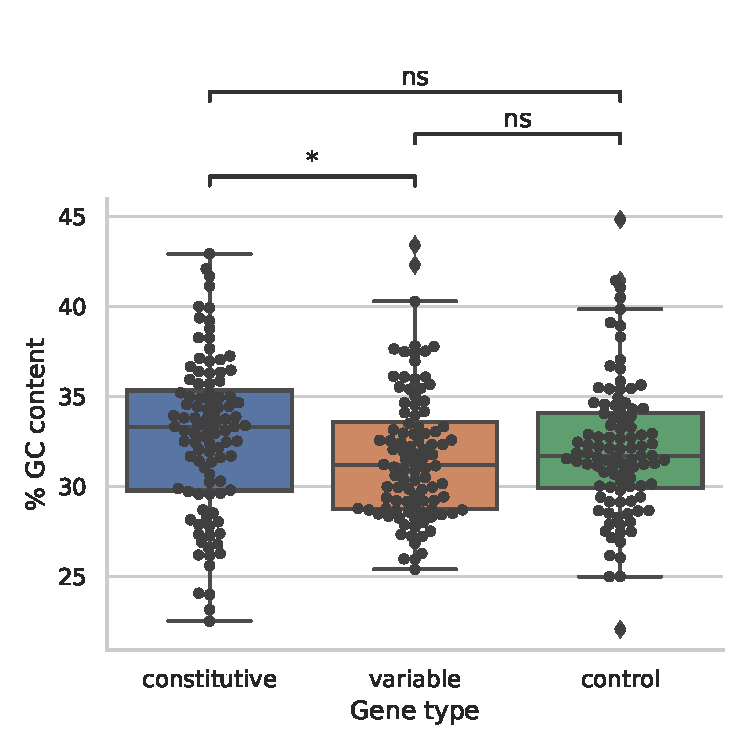
\includegraphics[width=0.50\columnwidth]{GC_content/wholeprom/Czechowski_GC_content_box}
		\caption{
			Percentage GC content of 100 constitutive (blue), 100 variable (orange) and 100 control (green) Arabidopsis \textit{cis}\hyp{}regulatory modules (CRMs).
			Promoters were extracted 1000 bp upstream of the annotated Araport 11 \autocite{chengAraport11CompleteReannotation2017} TSS or until the nearest gene.
			5UTRs were extended downstream of the TSS to the closest coding region.  Box plots have box boundaries that represent 25th, 50th (median) and 75th percentiles; whiskers are drawn up to the largest or smallest observed point that falls within 1.5 times the interquartile range.
			ns, not significant5.
			\label{fig:gc-content-wholeprom}
		}
	\end{center}
\end{figure}

A sliding window analysis revealed that within the first 400 bp upstream of the ATG start codon the median open chromatin was \SI{100}{\percent}.
This 400 bp region contained the majority of TSSs
Within this 400 bp region percentage GC content was higher for constitutive genes than variable genes (\autoref{fig:all-combined-sliding-window}C) and percentage bp covered by TFBSs was higher for variable genes than constitutive genes (\autoref{fig:all-combined-sliding-window}D). 50-100 bp upstream of the ATG start codon variable genes looked to have slightly higher Shannon diversity (\autoref{fig:all-combined-sliding-window}E).
From \textasciitilde{}350 bp to \textasciitilde{}600 bp upstream of the start codon the median open chromatin in constitutive CRMs decreases to zero while variable CRMs had a median percentage open chromatin of 0.
To confirm whether this was a genuine difference or due to different 5'UTR lengths between constutitive and variable genes, the percentage of root\hyp{}shoot intersect open chromatin of windows was plotted centred around the Araport11 TSS (\autoref{fig:all-combined-sliding-window-araporttss}).
The median percentage open chromatin decreased upstream of the TSS for both constitutive and variable genes, and constutive genes had a higher percentage open chromatin -100 to + 500 bp around the TSS (ADD STATS).%Add stats

%TALK ABOUT 5UTR lengths - test if constutive have longer 5'UTR lengths (check for expected  hypothesis first and see if useful comparison or not)
\begin{figure}[!h]
	\begin{center}
		\capstart
		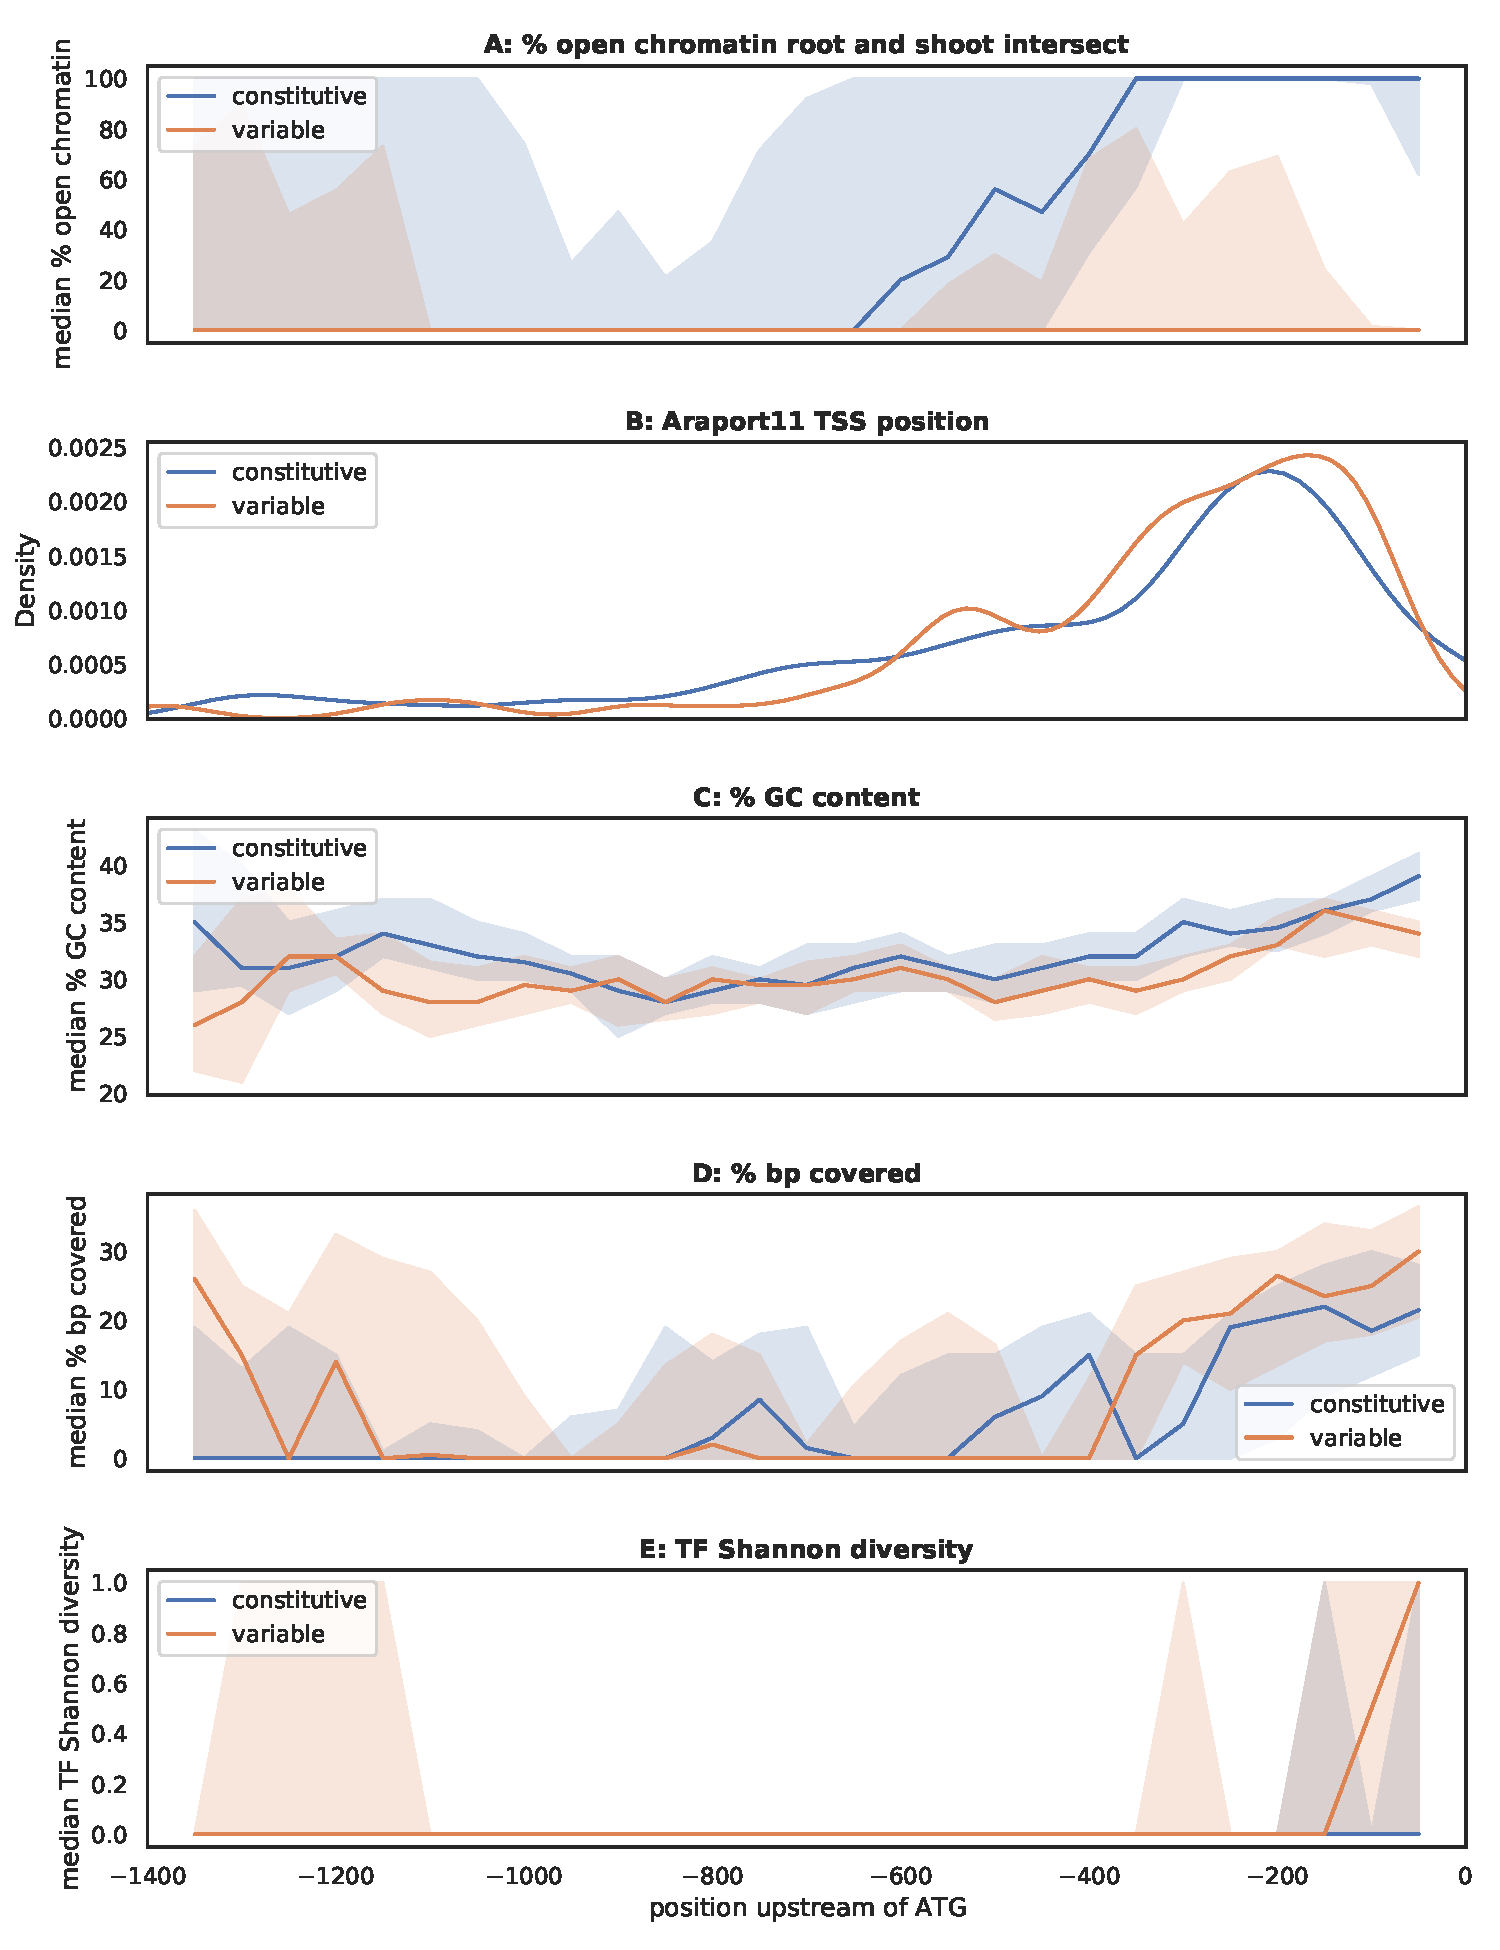
\includegraphics[width=1\columnwidth]{slidingwindow_combined/Czechowski_genetypenocontrol_all_combined_rw_median_sliding_window}
		\caption{
			Sliding window analysis of 100 constitutive (blue) and 100 variable (orange) Arabidopsis \textit{cis}\hyp{}regulatory modules (CRMs).
			Promoters were extracted 1000 base pairs (bp) upstream of the annotated Araport 11 \autocite{chengAraport11CompleteReannotation2017} TSS or until the nearest gene.
			5UTRs were extended downstream of the TSS to the closest coding region.
			Data points are positioned in the centre of each 100 bp window.
			Windows are offset by 50 bp.
			Shading represents 95 confidence intervals estimated using 10000 bootstraps.
			A: Median percentage of open chromatin peaks overlapping 100 bp windows. Open chromatin peaks derived from the intersect of root and shoot peaks derived from negative control (treated with NaOH) ATAC\hyp{}seq data by \textcite{potterCytokininModulatesContextdependent2018}.
			B: Position of Araport11 annotated transcription start site (TSS) upstream of the ATG start codon of the closest coding region.			
			C: Median percentage GC content in 100 bp windows. N = 95
			D: Median percentage bp covered by at least one transcription factor binding site.
			E: Shannon diversity of individual transcription factors binding within each 100 bp window.
			\label{fig:all-combined-sliding-window}
		}
	\end{center}
\end{figure}

\begin{figure}[!h]
	\begin{center}
		\capstart
		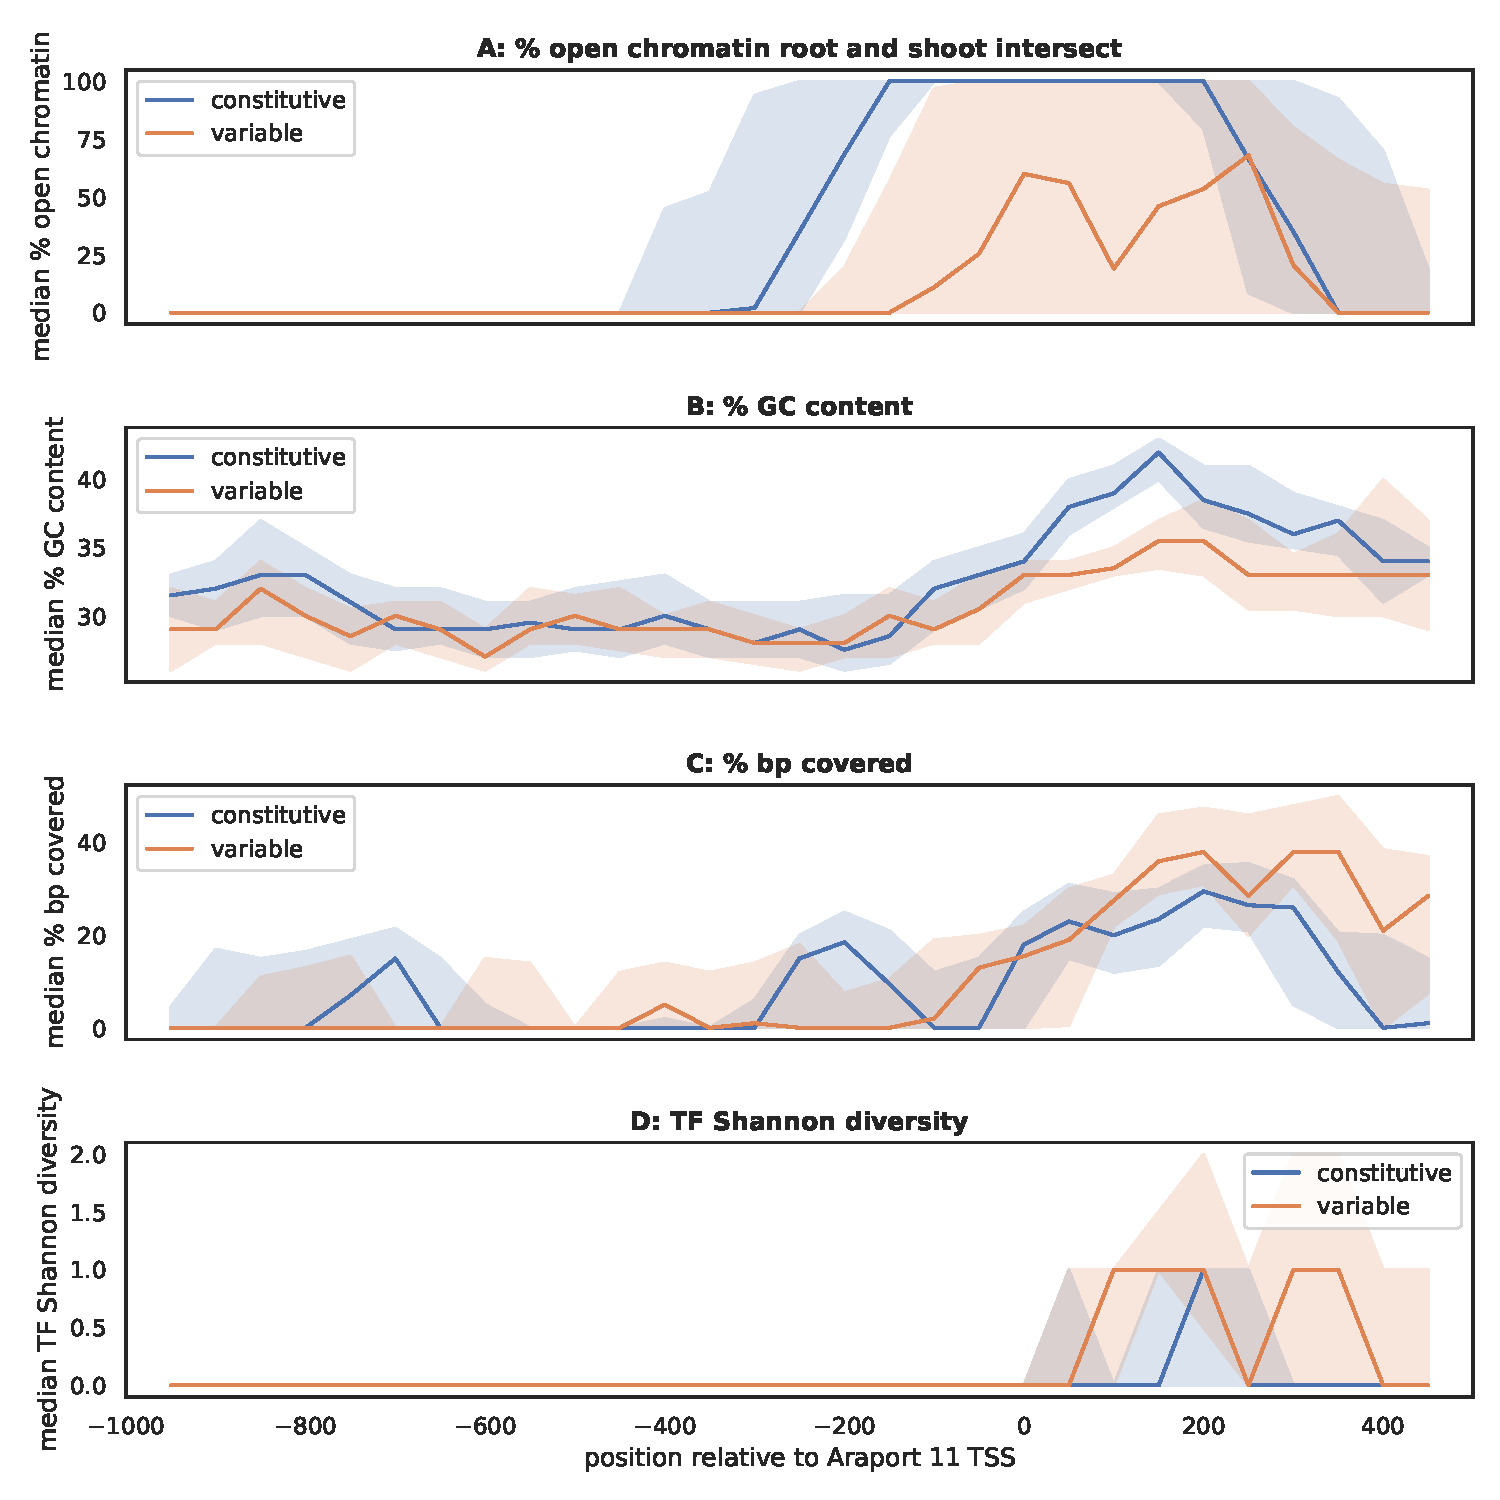
\includegraphics[width=1\columnwidth]{slidingwindow_combined/Araport11_Czechowski_genetypenocontrol_median_openchromatin_sliding_window}
		\caption{
			Sliding window analysis of 100 constitutive (blue) and 100 variable (orange) Arabidopsis \textit{cis}\hyp{}regulatory modules (CRMs). Promoters were extracted 1000 bp upstream of the annotated Araport 11 \autocite{chengAraport11CompleteReannotation2017} TSS or until the nearest gene.
			5UTRs were extended downstream of the TSS to the closest coding region.
			TSS is represented by 0 on the x-axis.
			Data points are positioned in the centre of each 100 bp window.
			Windows are offset by 50 bp.
			Shading represents 95 confidence intervals estimated using 10000 bootstraps.
			A: Median percentage of open chromatin peaks overlapping 100 bp windows. Open chromatin peaks derived from the intersect of root and shoot peaks derived from negative control (treated with NaOH) ATAC\hyp{}seq data by \textcite{potterCytokininModulatesContextdependent2018}.		
			B: Median percentage GC content in 100 bp windows.
			C: Median percentage bp covered by at least one transcription factor binding site.
			D: Shannon diversity of individual transcription factors binding within each 100 bp window.
			\label{fig:all-combined-sliding-window-araporttss}
		}
	\end{center}
\end{figure}






\begin{figure}[!h]
	\begin{center}
		\capstart
		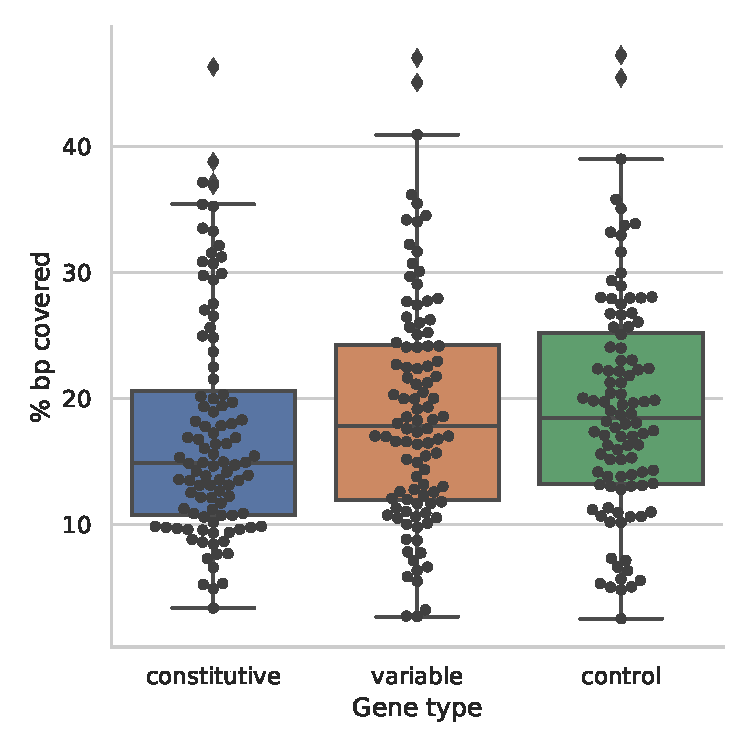
\includegraphics[width=0.50\columnwidth]{bp_covered/wholeprom/Czechowski_TFBS_coverage_box}
		\caption{
			The percentage of base pairs covered by at least one transcription
			factor binding motif in 100 constitutive (blue), 100 variable (orange) and 100 control (green)
			Arabidopsis \textit{cis}\hyp{}regulatory modules (CRMs). Promoters were extracted 1000 bp upstream of the
			annotated Araport 11 \autocite{chengAraport11CompleteReannotation2017} TSS or until the nearest gene. 5UTRs extended downstream of the TSS to the closest coding region.
			\label{fig:bp-covered-wholeprom}
		}
	\end{center}
\end{figure}
\end{document}